\documentclass[12pt]{article}
%\usepackage{tocloft}% to configure the ToC <<<<<
%\setlength{\cftsecnumwidth}{4.5ex}% set the width to the section number in the ToC <<<<<
%\renewcommand{\thesection}{\Roman{section}.} 
%\renewcommand{\thesubsection}{\quad \Alph{subsection}.}
%\renewcommand{\thesubsubsection}{\qquad \roman{subsubsection}.}

%\usepackage[style=authoryear,bibencoding=auto,strict,backend=biber,natbib,maxcitenames=2]{biblatex}

\usepackage{amssymb,amsmath,amsfonts,bbm,bm,dcolumn,booktabs,eurosym,geometry,ulem,graphicx,color,xcolor,setspace,sectsty,comment,float,caption,pdflscape,subfigure,array,hyperref}
\usepackage{xurl}
\usepackage[font=bf]{caption}
\usepackage[bottom]{footmisc}

\hypersetup{
    colorlinks,
    linkcolor={black},
    citecolor={blue!35!black},
    urlcolor={blue!35!black}
}
\normalem
\interfootnotelinepenalty=10000

\geometry{left=1.0in,right=1.0in,top=1.0in,bottom=1.0in}
\usepackage[style=authoryear,backend=bibtex,maxcitenames=2]{biblatex}
\addbibresource{biblio.bib}

\begin{document}
\title{Predicting Intraday Trading Volume with News Sentiment: An Analysis of U.S. Airline Stocks}
\author{Steven VanOmmeren\thanks{A complete replication package of this project is available at \url{https://github.com/svanomm/svo-directed-practicum}.}}
\date{\today}
\maketitle
\begin{abstract}
\noindent
    When institutional traders buy or sell large amounts of stock, they often have to consider the impact of their trades on the market price. Existing literature has shown that trading volume can be reliably forecasted and can translate to reduced price impact on large trades. In this paper, we attempt to model 15-minute ahead trading volume for 7 major U.S. airlines with a large set of financial variables as well as sentiment measures from the Global Database of Events, Language, and Tone (GDELT). Through a combination of feature engineering, model selection, and hyperparameter tuning, we achieve an out-of-sample $R^2$ of just over 70\% in the prediction of 15-minute ahead trading volume, over a testing period of approximately 18 months. This represents a significant improvement over a naive forecast, and is comparable with state-of-the-art models in the literature. We find that sentiment measures improve the model's predictions, but only marginally. These results suggest that sentiment measures are not necessary for accurate trading volume prediction, but they do not hurt the model's performance either. 
\end{abstract}
\doublespacing
\section{Introduction}
The commercial airline industry is somewhat unique in that information about adverse events streams nearly 24/7/365, is highly publicized, and has potential to dramatically affect public trust in the company. In today's digital world, news of a fatal plane crash typically appears online within an hour. Knowledge of a plane crash or other adverse event could significantly impact the airline's stock, either because the event reveals additional information to the public or because traders think that the event will matter. In addition, the general lack of after-hours trading for U.S. commercial airline stock allows real-time news sentiment to anticipate stock market movements.
    
    I examine the impact of such events on airline stock prices at the near-real-time level. Specifically, I leverage data from the Global Database of Events, Language, and Tone (GDELT) to scrape a rich set of sentiment measures from 1.3 million news articles mentioning the major U.S. commercial airlines.\footnote{\textcite{leetaru2013gdelt}.} I use these (and other) data to predict changes in stock volumes for 7 major U.S. airlines in 15-minute increments during the trading days from January 2018 to May 2025.

    This paper appears to be the first to publicly examine such a large volume of real-time GDELT data, the first to examine the effects of news sentiment on stock prices at a sub-daily level in the airline industry, and the first to consider the large set of supplemental sentiment indicators offered by GDELT for stock prediction. All of my code used to scrape and examine GDELT is available free and open-source, and can be used for business monitoring going forward.

\section{Literature Review}

\subsection{Stock Volume Prediction}
The fact that most traders are concerned with predicting stock prices makes stock prices nearly impossible to predict. An average day trader with access to the same (or worse) stock data as everyone else in the market is almost certainly unable to predict prices better than a firm employing hundreds or thousands of traders. However, predicting trading volumes (which do not provide direct information of prices) is a more attainable goal.

\textcite{goyenko2024trading} model the potential benefits associated with accurate predictions of trading volume. The authors explain that while trading volume is not particularly useful to a day trader, inaccurate forecasts of volume could lead a large trading firm to miscalculate the price impact of a trade. In the authors' theoretical model, overestimating the amount of trading volume when making a large trade would increase the net trading cost to the firm. Specifically, price impact is assumed to be proportional to the trade's share of total volume:
\begin{equation}
    |Price Impact_{t}| = \alpha\frac{v_{t}}{V_{t}}, \qquad 0< \alpha < 1,
\end{equation}
where $v_{t}$ is the volume of a given trade, and $V_{t}$ is the total volume of all trades at time $t$. The result is that buying (or selling) a large proportion of total volume makes the trade more costly, because price is higher (or lower) than it would be otherwise.The authors create a predictive model of changes in the log of dollar trading volume using technical indicators for 4700 stocks over a period of 1258 days. Their best model (an LSTM with 175 features) obtains an $R^2$ of around 20\% relative to the prediction accuracy of a moving average model. This demonstrates that, unlike stock price prediction, models can consistently predict daily trading volumes over a wide range of stocks.

\textcite{cucuringu2025forecasting} investigate the ability of machine learning models to predict intraday trading volumes. The authors analyze 15-minute data over a period of 6 months for each constituent stock in the S\&P 500 index. A baseline model is able to predict out-of-sample volumes with an $R^2$ of 0.265, while their best model attains an $R^2$ of 0.624. The authors then demonstrate the usefulness of their model for large traders seeking to minimize the price impact of a trade. Their model improves the volume-weighted average price (VWAP) order execution risk for a sample of 5 stocks by an average of around 29\%, compared to a baseline model.

\textcite{satish2014predicting} make the case for using a statistical model to predict trading volumes. The authors explain that at the time,  the typical approach taken by firms was to just use moving averages of trading volumes as a predictor. The authors combine two ARMA models with varying levels of historical data (intraday and daily) to predict trading volume. After calibrating their model, the authors were able to increase VWAP error performance by 9\% compared to the typical moving average approach. Notably, the authors explain that news events can affect VWAP tracking error, though they do not include news sentiment in their model.
\subsection{GDELT}
Previous studies have assessed the usefulness of GDELT for predicting stock prices. However, apparently all of them have aggregated GDELT to a daily level, rather than using it at its original real-time 15-minute increments. To my knowledge, only one study has taken advantage of the GDELT sentiment measures outside of the basic metrics of Tone, count of articles, and number of positive/negative sentiment words for predicting financial markets.

\textcite{nashir2023indonesian} incorporate GDELT data into a machine learning model to predict stock prices. The authors source a long span of daily stock data from Jan. 2008 to Dec. 2022 (5479 observations), specifically for the Jakarta Stock Exchange (JKSE) index of Indonesian stocks. The authors study 4 sentiment measures using GDELT data: tone, optimism, attention, and tone dispersion. These metrics are calculated at the daily level. The authors then train a modified version of an LSTM model using time series cross-validation. The authors document an extensive hyperparameter optimization, which yielded an improved model with a mean absolute percentage error (MAPE) of 0.8\%. They additionally find that a model trained with only the ``optimism" feature slightly outperforms the model with all four sentiment measures.\footnote{The combined model outperforms the other models that include only a single sentiment metric (tone, attention, or tone dispersion).} The authors do not compare their results to a Naive forecast.

\textcite{wang2024ensemble} use GDELT data to inform the prediction of a variety of individual stocks and indices. They do not identify articles specific to each stock, instead summing the number of article mentions and the sum of Tone for each CAMEO code. CAMEO codes provide high-level descriptions of conflict identified in an article, e.g. ``Threaten" or ``Engage in political dissent." The authors then evaluate causal relationships between the CAMEO-specific metrics with each stock price at the daily level from Jan. 2018 to Feb. 2022. These causal relationships are incorporated into an LSTM model to predict stock prices. The authors report that this model performs best out of a variety of other models (including ARIMA, VAR, etc.). Unfortunately, the authors do not compare the performance of their model to a Naive prediction, and a close look at their Figures 9 and 10 shows that their best model essentially predicts the previous stock price. In other words, they likely do not beat a Naive forecast.

\textcite{consoli2021information} assess the use of GDELT for modeling sovereign spreads in the European bond market. The time series of interest is the sovereign spread of Italy vs Germany with respect to 10-year bond yields, with 468 data points covering a time period of Mar. 2015 to Aug. 2019. The authors filtered GDELT to identify articles specific to macroeconomic discussions in the locations of interest. They identify a subset of 45 GDELT variables that are both quantitatively and qualitatively relevant to bond markets. The authors then include these variables along with bond market data in a probabilistic LSTM model, yielding an out-of-sample R-squared of 0.23 for predicting changes in the dependent variable. While the study suffers from a small sample size and does not compare its accuracy to a Naive forecast, it provides robust evidence that GDELT could be useful for predicting bond markets.

\textcite{jakel2019using} investigates correlations between GDELT sentiment and the stock prices of U.S. technology companies. The author sourced approximately 60,000 articles over a 29-day period in 2019. He then averaged the sentiment Tone by company and day to join to 29 days of stock price data for Facebook, Apple, Amazon, Alphabet and Tesla. Analyzing the correlation between sentiment and stock price, the author found a generally contrarian relationship. However, the results are inconclusive due to a small sample size.

\textcite{alamro2019predicting} use GDELT's Tone and count of articles per day to predict TASI, a Saudi stock market index. The authors filtered GDELT data to any articles that mention Saudi Arabia, then aggregate the data to the daily level, averaging the Tone metric and counting the number of articles per day. The authors then test a variety of models to predict the index price, finding that an LSTM model performs dramatically better than more traditional forecasting models. Unfortunately, the authors do not report the specification of the LSTM model, any scale-independent measures of model fit, any comparisons to a Naive forecast, any tests of whether the sentiment measures add predictive value, nor any graphs of predicted vs actual stock prices. It is therefore unclear whether the authors' LSTM model provides better-than-Naive performance or if the sentiment measures actually improved the fit of the model.

\section{Methods}
Below, we explain the data preparation and modelling techniques used to evaluate the usefulness of GDELT for predicting airline stock volume.\footnote{All processing and modelling was performed on a Windows 10 desktop with the following specifications: 128GB of DDR4 RAM, an Nvidia RTX 2070 Super (8GB VRAM), and an AMD Ryzen 5 3600 processor. Some of the computations described below likely would not run on anything less than 128GB of RAM without modification.}
\subsection{Data Preparation}
\subsubsection{GDELT}
GDELT offers a variety of databases to the public. For this analysis, we use the Global Knowledge Graph version 2 (GKG). For each article identified by GDELT, the GKG reports:
\begin{itemize}
\singlespacing
    \item the date scraped by GDELT (at the 15-minute level)
    \item the article URL (or other unique identifier)
    \item every location, business, and important person named in the article text
    \item Conflict and Mediation Event Observations (CAMEO) codes identified in the article
    \item 7 sentiment measures based on the article text (Tone, Positive Score, Negative Score, Polarity, Activity Reference Density, Self/Group Reference Density, Word Count). These are called the GKG1 sentiment measures
    \item 111 additional sentiment measures that use a scored value (called the GKG2 scored measures)
    \item 2878 additional sentiment measures that use word count (called the GKG2 word count measures)
    \item the article headline text (if available).\footnote{GDELT only started scraping the article headline in Sep. 2019. Prior to this time, we recover part of the article headline using the URL, which often contains a relevant description of the story.}
\end{itemize}
Importantly, GDELT does \textit{not} store the article text itself. GDELT uploads the raw GKG data in separate files every 15 minutes. These files are available to download for free, but the full combined data is available to query in Google BigQuery for a fee. The files are saved at the article level, i.e. the articles that GDELT scraped in a given 15-minute period.

Because the combined data is several tens of terabytes (TBs), we did not have the storage capacity to save all the raw data. Instead, we filtered the raw files to articles matching the airline industry before saving the data. The general outline of our data processing is:
\begin{itemize}
\singlespacing
    \item access and unzip the raw file for a given 15-minute period
    \item keep a limited subset of columns from the raw file
    \item limit to articles mentioning a location of ``United States"
    \item limit to articles that mention at least one of the following organizations: Alaska Airlines, American Airlines, Delta Air Lines, Frontier Airlines, Hawaiian Airlines, JetBlue, Southwest Airlines, Spirit Airlines, Sun Country Airlines, United Airlines, Allegiant Air
    \item drop articles that are missing any key fields
\end{itemize}
We repeated this process for the approximately 260,000 15-minute periods covering the timeline of 1/1/2018 00:00:00 to 5/30/2025 23:45:00. Data downloading was performed over multiple several-hour periods, and was parallelized to increase download speeds. After filtering, 218,574 raw GDELT files were combined for a total of 1,261,785 articles identified.\footnote{The total raw GDELT files kept is less than the theoretical 260,000 files for multiple reasons, including: no airlines mentioned in the past 15 minutes, and sporadic GDELT outages.}

Next, we performed extensive data cleaning to filter the articles to those that would likely affect the stock market:
\begin{itemize}
\singlespacing
    \item restricting the sentiment indicators to finance- and economics-specific measures
    \item removing frequent article titles that relate to the front page of a news site (rather than a specific article) or an unrelated article
    \item restricting to top news websites (e.g. MSN, Reuters) and finance-related websites (e.g. Investors.com)
    \item removing discussions of historical airline events (such as the September 11 attacks)
    \item removing articles that did not have a valid article title after data processing
    \item removing a small set of duplicate articles\footnote{Duplicate articles are likely due to the data downloading process, which was stopped and restarted multiple times.}
\end{itemize}
After cleaning and filtering, we have 121,655 relevant articles and 118 sentiment measures.

To extract additional sentiment from the GDELT data, we use a \textbf{Large Language Model} (LLM) to embed the article titles in a high-dimensional vector space. We apply a 596-million parameter embedding model to each article title.\footnote{\url{https://huggingface.co/Qwen/Qwen3-Embedding-0.6B}. This embedding model optionally takes an instruction prompt as an input. We use the following prompt for our embeddings: \textsf{Instruct: Extract the sentiment from this news headline that is most likely to affect the airline stock market. Query:}.} The model is trained to output 1024-dimensional vectors, however we use the Matryoshka Transformer (MatFormer) method to truncate the vectors to 32 dimensions, acting as a dimensionality reduction technique. These 32 dimensions are then used as additional sentiment measures in the model.

After constructing the sentiment measures, we aggregate the data to align with stock market data and to identify sentiment scores separately by airline. Each metric is interacted with a set of indicator variables identifying the airline companies.\footnote{Multiple airlines can be mentioned in the same article, in which case the article is included each of the airlines' interacted sentiment values.} We then sum the metrics by 15-minute interval and fill in missing time periods with zeroes.\footnote{GDELT data is recorded in the UTC timezone, while my stock data is in EST. I converted the timezone before merging these datasets.} At this point, the GDELT data is in 15-minute intervals, but it includes times outside of market open. We further aggregate the data to align with market open. The choice of aggregation strategy is not obvious here. The number of observations to aggregate influences the scale of the resulting sentiment scores. Summing a particular window of observations (e.g. 2 hours) assumes that sufficient information is captured in that time period for predicting stock behavior.\footnote{Note that simply collapsing all of the market close data into one observation would result in large sentiment values at market open, and small values for the rest of the trading day. This would essentially vanish any effects of events that occur during the trading day.} We address this issue by calculating rolling sums over varying time windows: 1 hour, 4 hours, 12 hours, and 24 hours. These sums influence the non-after-hours observations as well, making them essentially moving averages. Each of these rolling sums is included in the feature set to allow the model to identify combinations of windows that best fit the data.

After calculating the rolling sums for each airline, metric, and window, we calculate the first lag of each variable to ensure that they can be used for out-of-sample predictions. Finally, the data is reshaped so that each observation is a 15-minute-bin and stock ticker. The final data has 338,324 rows and 750 sentiment features.

\subsubsection{Stocks}
Stock data were downloaded in 15-minute increments during market open from Barchart, for the period Jan. 2018 to May 2025. The following tickers were downloaded:
\begin{itemize}
\singlespacing
    \item AAL: American Airlines Group Inc.
    \item ALGT: Allegiant Travel Company
    \item ALK: Alaska Air Group Inc.
    \item DAL: Delta Air Lines Inc.
    \item JBLU: JetBlue Airways Corp.
    \item LUV: Southwest Airlines Co.
    \item UAL: United Airlines Holdings Inc.
    \item BNO: United States Brent Oil Fund LP
    \item ITA: iShares US Aerospace \& Defense ETF
    \item IYT: iShares US Transportation ETF
    \item JETS: US Global Jets ETF
\end{itemize}
As seen from the list, we include some stocks as control variables that are likely correlated with airline stocks: 3 airplane-related ETFs, and an oil fund. The raw data include the stock's open, high, low, and last price, and volume traded over each 15-minute period. We calculate additional features for each stock:
\begin{itemize}
\singlespacing
    \item High-Low spread (in levels and percentage)
    \item Last-Open spread (in levels and percentage)
    \item 1-period change in open, high, low, last price, and volume
    \item Change in trading volume compared to same time on previous trading day (10 lags)
    \item 10-period rolling standard deviation of last price
    \item 10-period rolling standard deviation of volume
    \item 10-period rolling standard deviation of the 10-period SD of price
    \item 10-period rolling standard deviation of the 10-period SD of volume
\end{itemize}
The last 4 measures are meant to capture changes in volatility for a given stock.

We then calculate a variety of moving averages for each metric, with the following windows: 4 periods (1 hour), 8 periods (2 hours), 16 periods (4 hours), and 26 periods (one trading day). For price, volume, change in price, and change in volume, we also calculate 26 periods of 15-minute lags. The data is reshaped so that each observation is a 15-minute bin and stock ticker (for the 7 airline stocks). The features include the stock's own set of features (self-finance), as well as the features of the ETFs and oil fund. The final data has 337,795 rows and 800 lagged features for prediction.

The GDELT and stock data are merged by 15-minute bin and stock ticker. As a final step, we create indicator variables for each hour of day, day of week, and month of year, as well as indicators for market open and market close. These indicators are meant to capture multilevel seasonality common across the stocks.

\subsection{Modeling}

We test a variety of models on multiple subsets of the features described above to understand which features contribute the most to predicting stock volume. We create the following feature sets:
\begin{itemize}
\singlespacing
    \item \textbf{Time Only}: open/close, hour of day, day of week, and month of year indicators (26 features)
    \item \textbf{Sentiment Only}: 118 GDELT measures, 32 LLM measures, with 1 non-moving average and 4 moving averages (750 features)
    \item \textbf{Self-Finance Only}: the respective stock's financial features discussed above (includes lags and moving averages) (160 features)
    \item \textbf{Finance Only}: self-finance features plus the features for the 3 ETFs and 1 oil fund (800 features)
    \item \textbf{Finance + Time}: all finance features plus the time indicators (826 features)
    \item \textbf{All Features}: (1576 features)
\end{itemize}
We then test the following models on each of these feature sets, where the dependent variable is the trading volume of the respective stock in a 15-minute bin:\footnote{All models were run using the \textsf{scikit-learn} package in Python. \textcite{scikit-learn}.}
\begin{itemize}
\singlespacing
    \item \textbf{OLS}: a standard linear regression, which is an ARMA model in some feature sets
    \item \textbf{LASSO}: a linear regression with LASSO regularization, which is an ARMA model in some feature sets. The penalty term $\alpha$ is set to 1.
    \item \textbf{Neural Network}: a fully-connected feed-forward neural network with 2 hidden layers, each with 20 neurons.\footnote{We experimented with alternative architectures but ultimately decided on a relatively small architecture to reduce overfitting and for computational reasons. Additional performance would come from tuning the architecture for each feature set, which we did not do here.} The activation function is ReLU, and the output layer uses a linear activation function.
    \item \textbf{LightGBM}: a histogram-based gradient boosting tree model.\footnote{\textcite{ke2017lightgbm}.} We do not tune the hyperparameters for each feature set. We found via experimentation that the following settings gave sufficient performance: no $L2$ regularization, no dropout, minimum of 200 samples per leaf, with no maximum depth or maximum leaf nodes. Early stopping was used to prevent overfitting,\footnote{Specifically, training was stopped if the model's $R^2$ on the validation set failed to improve for 10 iterations.} with a maximum of 2000 iterations.
\end{itemize}
Each of these models was trained on a training subset of the data (the first 80\% of observations sorted by time and ticker), and evaluated on both a validation set (the next 10\% of observations) and a test set (the final 10\% of observations). Because the machine learning models are sensitive to the scale of features, we normalize each feature to the interval $[0,1]$ using a min-max scaler.

\subsection{Hyperparameter Tuning}
Hyperparameter tuning is the process of changing some of the input settings in the model to optimize its performance. Overfitting is a particular concern for the full feature set, with over 1500 features. To reduce computational cost, we only tuned the LightGBM model with all features included. Rather than a traditional grid search, we used a Bayesian optimization approach via the Optuna library to find the best hyperparameters.\footnote{\textcite{optuna_2019}.} The hyperparameters tuned were:\footnote{These models were trained with a learning rate of 0.1, which was found to provide a good tradeoff between training speed and performance.}
\begin{itemize}
\singlespacing
    \item \textbf{min samples per leaf}: the minimum number of samples required per leaf node. We tested values from 100 to 10000 on a logarithmic scale.
    \item \textbf{L2 regularization}: a regularization penalty term. We tested values from 0 to 3 on a uniform scale.
    \item \textbf{max features}: the maximum proportion of features shown to the model during training. We tested values from 0.05 to 1.0 on a uniform scale.
\end{itemize}
Each of these hyperparameters acts as a regularization term, preventing the model from overfitting to the training data. Optuna tuned the hyperparameters with the objective of maximizing the average out-of-sample $R^2$ on both the validation and testing sets. Tuning was run for approximately 6 hours, resulting in 65 trials. The best hyperparameters were then used to train the final model with a lower learning rate and more iterations. The final model was retrained with a lower learning rate of 0.005, 10000 iterations, and the best hyperparameters found by Optuna.

\section{Results and Analysis}
\subsection{Summary Analysis}
\subsection{Correlation Analysis}
\subsubsection{Contemporaneous Correlation}
First, Figure \ref{fig:contemp_open} reports the contemporaneous correlation in first-differences of open price for the airline stocks of interest. Correlations are calculated using the 15-minute data.
\begin{figure}[H]
    \centering
    \caption{Contemporaneous Correlation, Change in Open Price}
%    \includegraphics[width=0.75\linewidth]{Figures/Contemporaneous_Open.png}
    \label{fig:contemp_open}
\end{figure}
Next, Figure \ref{fig:contemp_vol} reports the contemporaneous correlation in first-differences of trading volume for the airline stocks of interest.
\begin{figure}[H]
    \centering
    \caption{Contemporaneous Correlation, Change in Trading Volume}
 %   \includegraphics[width=0.75\linewidth]{Figures/Contemporaneous_Volume.png}
    \label{fig:contemp_vol}
\end{figure}
These figures show that the airline stocks exhibit a substantial and positive correlation. The airline-relevant indices (ITA, IYT, and JETS) have lower but still-relevant positive correlations. 

\subsubsection{Lagged Correlation}
Next, I report the correlations among the lag of these variables. Figure \ref{fig:lagged_open} reports correlations between a stock's change in price at time $t$ (the rows) with a stock's change in price at time $t-1$ (the columns). For example, the diagonal entries report the first-order autocorrelation of each stock.
\begin{figure}[H]
    \centering
    \caption{Lagged Correlation, Change in Open Price}
 %   \includegraphics[width=0.75\linewidth]{Figures/Lagged_Open.png}
    \label{fig:lagged_open}
\end{figure}
Similarly, Figure \ref{fig:lagged_volume} reports the correlations among changes in trading volumes.
\begin{figure}[H]
    \centering
    \caption{Lagged Correlation, Change in Trading Volume}
    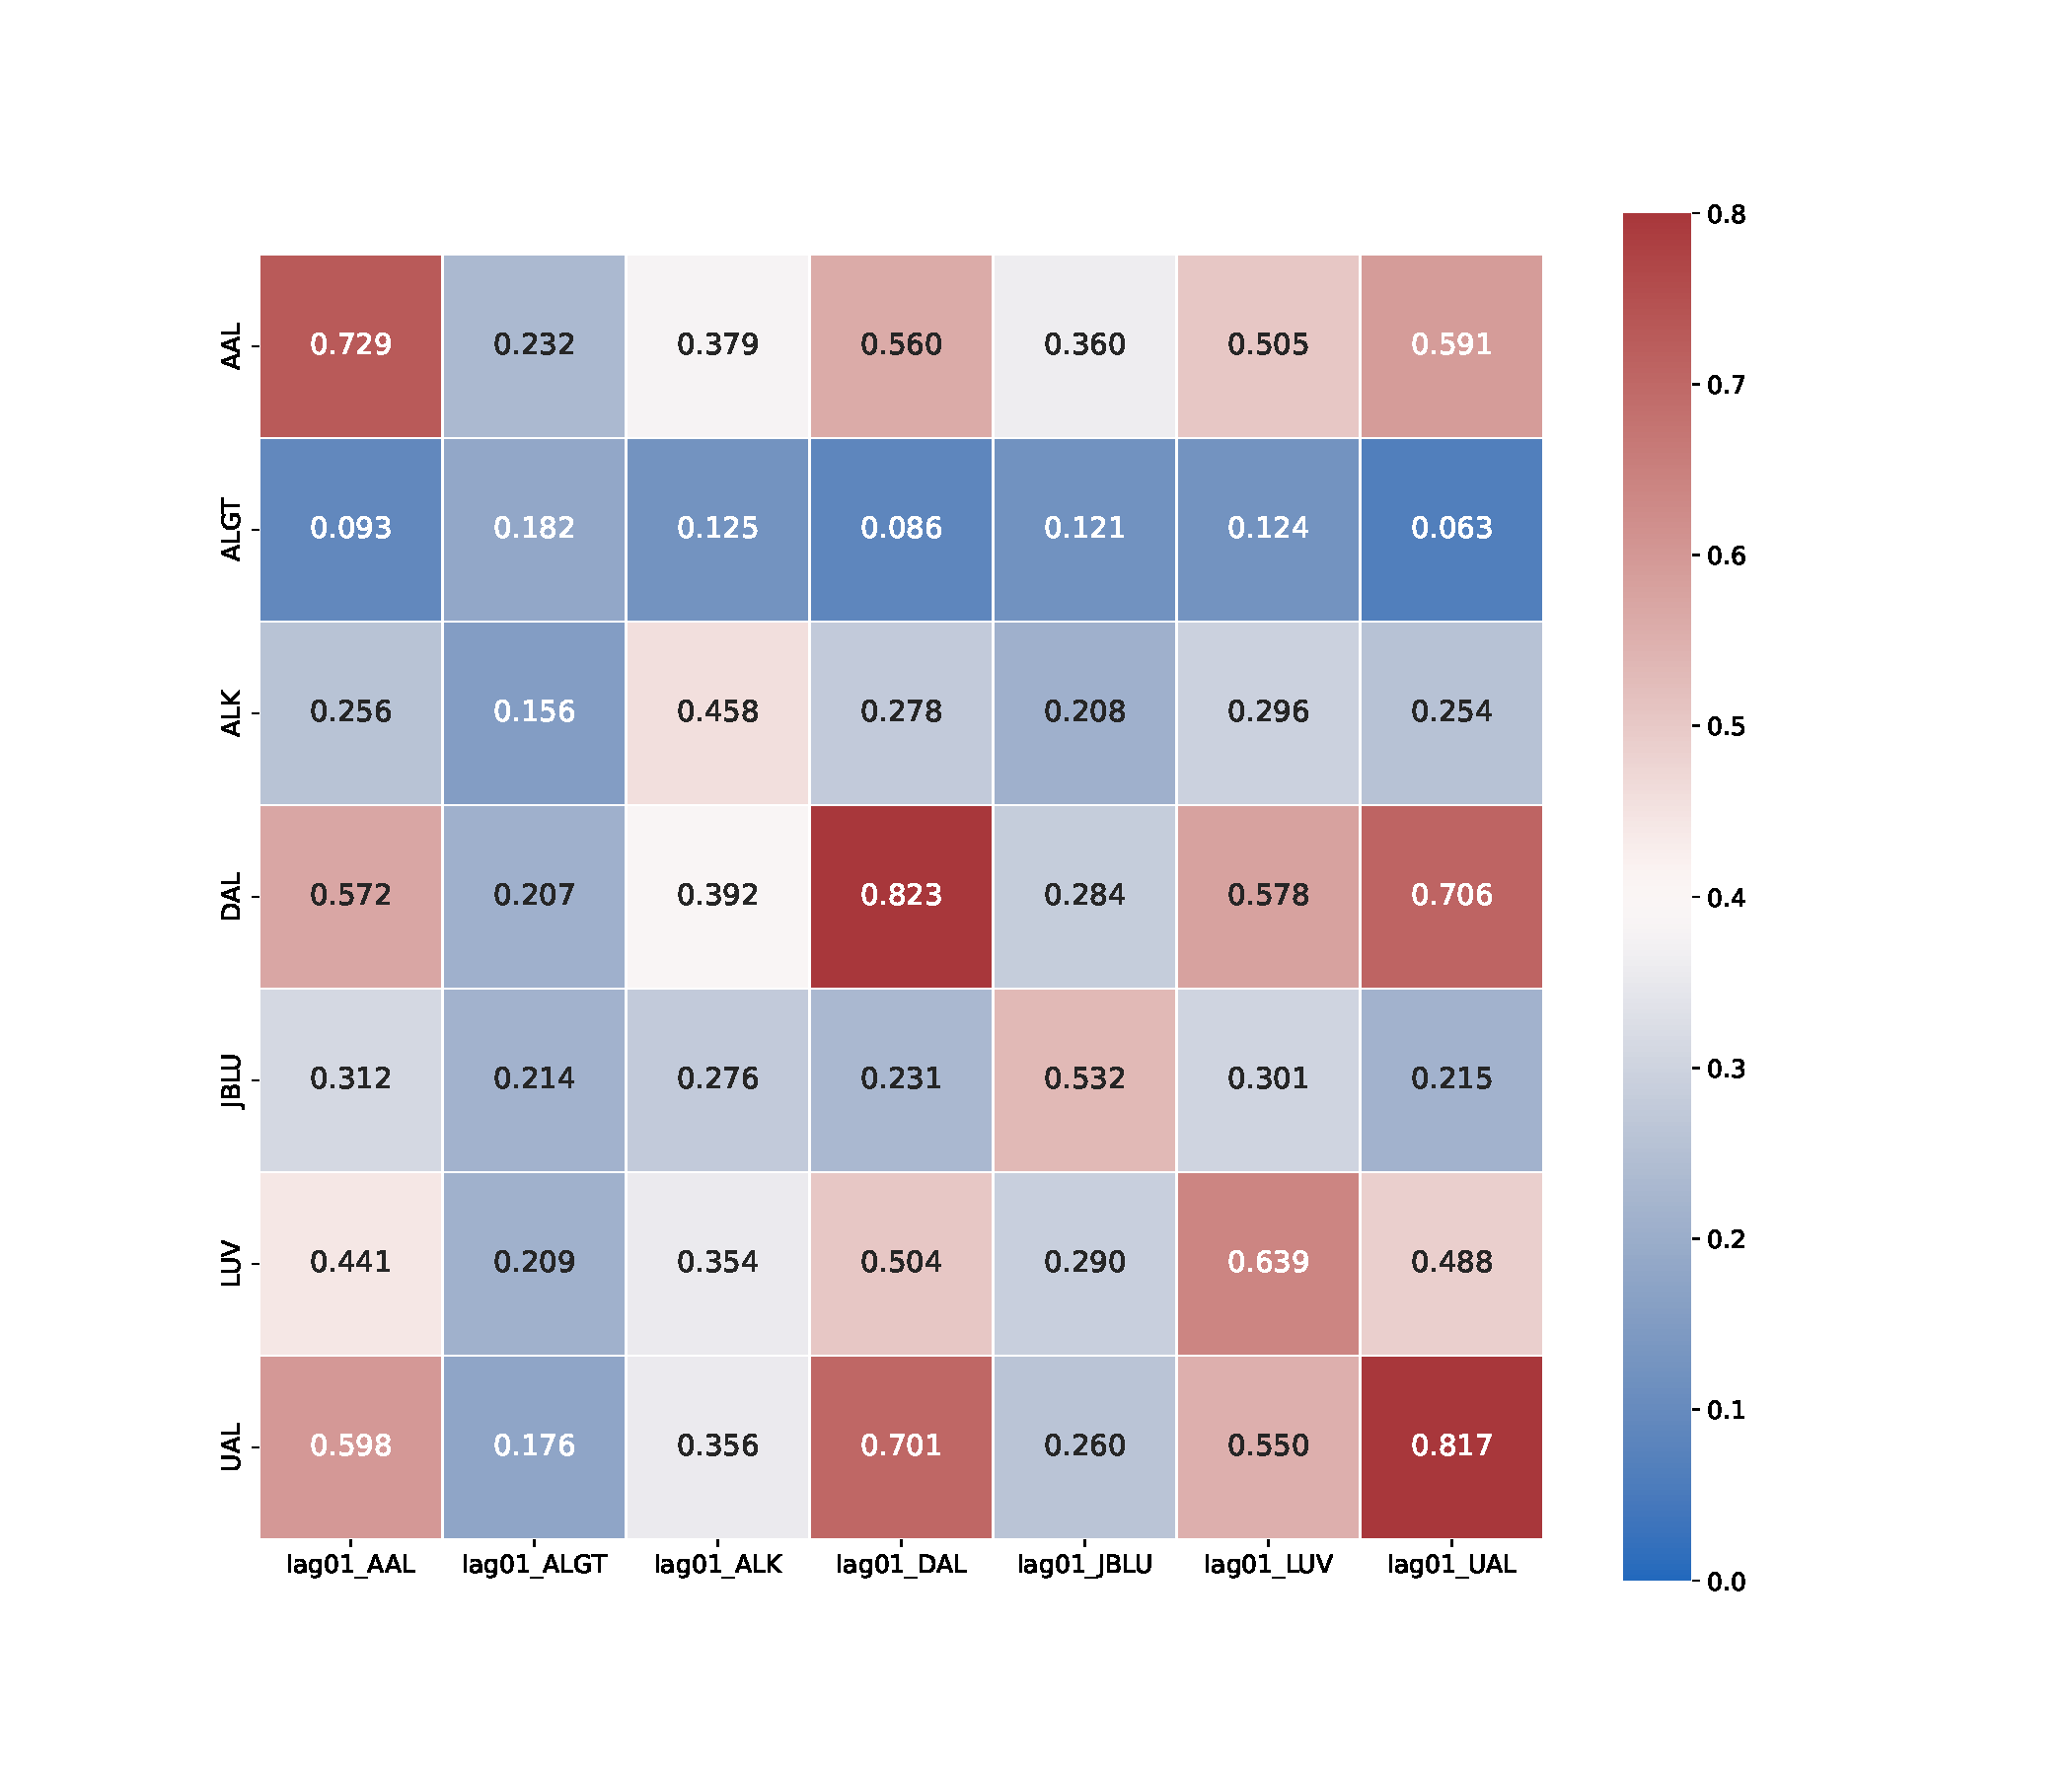
\includegraphics[width=0.75\linewidth]{../Output/Correlation Matrices/Lagged_Volume.png}
    \label{fig:lagged_volume}
\end{figure}
Due to the highly unpredictable nature of the stock market, these correlations are much smaller. For example, United Airlines and Delta Airlines have a contemporaneous correlation of 0.83 with respect to price changes, but lagged price changes for Delta have only a 0.038 correlation with current price changes for United.

While the lagged correlations for prices are mostly positive, the lagged correlations in trading volume are almost all negative, a reversal compared to the contemporaneous chart.


\subsection{Models}
Before reporting the model results, we establish a baseline model. Similar to \textcite{goyenko2024trading}, we use a simple average of the trading volume for the past 5 days as a baseline predictor of volume.\footnote{Specifically, we use the 15-minute volume at the same time of the previous 5 trading days. The model comes from an OLS regression of volume on the average historical volume, plus a constant.} This simple model performs quite well, with an out-of-sample $R^2$ of just under 0.56 over the entire testing period.

\begin{table}[H]
\caption*{
{\large Out-of-Sample 15-Minute-Ahead Volume Prediction} \\
{\small $R^2$ Values, All Stocks, 2023-12-04 to 2025-05-30}
} 

\fontsize{12.0pt}{14.4pt}\selectfont

\begin{tabular*}{\linewidth}{@{\extracolsep{\fill}}lrrrr}
\toprule
Features & OLS & LASSO & Neural Network & LightGBM \\ 
\midrule\addlinespace[2.5pt]
Time Only & 0.0973 & 0.0973 & 0.0916 & 0.0978 \\
Sentiment Only & 0.0079 & 0.0314 & -0.0418 & 0.0762 \\
Self-Finance Only & 0.6330 & 0.6325 & 0.5912 & 0.6817 \\
Finance Only & 0.6361 & 0.6363 & 0.5702 & 0.6865 \\
Finance + Time & 0.6441 & 0.6444 & 0.6388 & 0.6893 \\
All & 0.6478 & 0.6492 & 0.6389 & 0.6952 \\
All (Tuned) &  &  &  & 0.7000 \\
All (Tuned, Retrained) &  &  &  & 0.7007 \\
\bottomrule
\end{tabular*}
\begin{minipage}{\linewidth}
Note: Models trained on data from 2018-01-02 to 2023-12-04.\\
\end{minipage}
\end{table}


\newpage
\section{Discussion}

As shown in the table above, adding the sentiment indicators improves each model's performance, but only marginally so. The best-performing model (LightGBM), improves its $R^2$ from 0.6893 to 0.6952 when incorporating the sentiment indicators into the model, not even a 1 percentage point increase. While it is an improvement, the lack of a large increase in performance suggests that historical financial data absorbs nearly all relevant sentiment information. While a financial institution seeking the most accurate forecasts may want to use GDELT's sentiment data as part of their volume forecasting, the data collection and curation costs are likely not worth the marginal increase in performance. On the contrary, the stock and other financial data are available at much lower cost and do not require the same level of curation.

\section{Conclusion}
The model results confirm that stock volume can be accurately forecasted better than a baseline model using historical averages. However, the results also show that sentiment measures add little additional content beyond historical financial information. This suggests that costly sentiment data curation may not be necessary for better-than-baseline stock volume prediction. However, financial institutions seeking the absolute best performance may want to include sentiment measures to get a small boost in forecasting accuracy.

\newpage
\printbibliography
\end{document}